% Options for packages loaded elsewhere
\PassOptionsToPackage{unicode}{hyperref}
\PassOptionsToPackage{hyphens}{url}
%
\documentclass[
  ignorenonframetext,
]{beamer}
\usepackage{pgfpages}
\setbeamertemplate{caption}[numbered]
\setbeamertemplate{caption label separator}{: }
\setbeamercolor{caption name}{fg=normal text.fg}
\beamertemplatenavigationsymbolsempty
% Prevent slide breaks in the middle of a paragraph
\widowpenalties 1 10000
\raggedbottom
\setbeamertemplate{part page}{
  \centering
  \begin{beamercolorbox}[sep=16pt,center]{part title}
    \usebeamerfont{part title}\insertpart\par
  \end{beamercolorbox}
}
\setbeamertemplate{section page}{
  \centering
  \begin{beamercolorbox}[sep=12pt,center]{part title}
    \usebeamerfont{section title}\insertsection\par
  \end{beamercolorbox}
}
\setbeamertemplate{subsection page}{
  \centering
  \begin{beamercolorbox}[sep=8pt,center]{part title}
    \usebeamerfont{subsection title}\insertsubsection\par
  \end{beamercolorbox}
}
\AtBeginPart{
  \frame{\partpage}
}
\AtBeginSection{
  \ifbibliography
  \else
    \frame{\sectionpage}
  \fi
}
\AtBeginSubsection{
  \frame{\subsectionpage}
}
\usepackage{lmodern}
\usepackage{amssymb,amsmath}
\usepackage{ifxetex,ifluatex}
\ifnum 0\ifxetex 1\fi\ifluatex 1\fi=0 % if pdftex
  \usepackage[T1]{fontenc}
  \usepackage[utf8]{inputenc}
  \usepackage{textcomp} % provide euro and other symbols
\else % if luatex or xetex
  \usepackage{unicode-math}
  \defaultfontfeatures{Scale=MatchLowercase}
  \defaultfontfeatures[\rmfamily]{Ligatures=TeX,Scale=1}
\fi
\usetheme[]{metropolis}
% Use upquote if available, for straight quotes in verbatim environments
\IfFileExists{upquote.sty}{\usepackage{upquote}}{}
\IfFileExists{microtype.sty}{% use microtype if available
  \usepackage[]{microtype}
  \UseMicrotypeSet[protrusion]{basicmath} % disable protrusion for tt fonts
}{}
\makeatletter
\@ifundefined{KOMAClassName}{% if non-KOMA class
  \IfFileExists{parskip.sty}{%
    \usepackage{parskip}
  }{% else
    \setlength{\parindent}{0pt}
    \setlength{\parskip}{6pt plus 2pt minus 1pt}}
}{% if KOMA class
  \KOMAoptions{parskip=half}}
\makeatother
\usepackage{xcolor}
\IfFileExists{xurl.sty}{\usepackage{xurl}}{} % add URL line breaks if available
\IfFileExists{bookmark.sty}{\usepackage{bookmark}}{\usepackage{hyperref}}
\hypersetup{
  pdftitle={Introduction to Data Science},
  pdfauthor={CSC/ST 442},
  hidelinks,
  pdfcreator={LaTeX via pandoc}}
\urlstyle{same} % disable monospaced font for URLs
\newif\ifbibliography
\usepackage{color}
\usepackage{fancyvrb}
\newcommand{\VerbBar}{|}
\newcommand{\VERB}{\Verb[commandchars=\\\{\}]}
\DefineVerbatimEnvironment{Highlighting}{Verbatim}{commandchars=\\\{\}}
% Add ',fontsize=\small' for more characters per line
\usepackage{framed}
\definecolor{shadecolor}{RGB}{248,248,248}
\newenvironment{Shaded}{\begin{snugshade}}{\end{snugshade}}
\newcommand{\AlertTok}[1]{\textcolor[rgb]{0.94,0.16,0.16}{#1}}
\newcommand{\AnnotationTok}[1]{\textcolor[rgb]{0.56,0.35,0.01}{\textbf{\textit{#1}}}}
\newcommand{\AttributeTok}[1]{\textcolor[rgb]{0.77,0.63,0.00}{#1}}
\newcommand{\BaseNTok}[1]{\textcolor[rgb]{0.00,0.00,0.81}{#1}}
\newcommand{\BuiltInTok}[1]{#1}
\newcommand{\CharTok}[1]{\textcolor[rgb]{0.31,0.60,0.02}{#1}}
\newcommand{\CommentTok}[1]{\textcolor[rgb]{0.56,0.35,0.01}{\textit{#1}}}
\newcommand{\CommentVarTok}[1]{\textcolor[rgb]{0.56,0.35,0.01}{\textbf{\textit{#1}}}}
\newcommand{\ConstantTok}[1]{\textcolor[rgb]{0.00,0.00,0.00}{#1}}
\newcommand{\ControlFlowTok}[1]{\textcolor[rgb]{0.13,0.29,0.53}{\textbf{#1}}}
\newcommand{\DataTypeTok}[1]{\textcolor[rgb]{0.13,0.29,0.53}{#1}}
\newcommand{\DecValTok}[1]{\textcolor[rgb]{0.00,0.00,0.81}{#1}}
\newcommand{\DocumentationTok}[1]{\textcolor[rgb]{0.56,0.35,0.01}{\textbf{\textit{#1}}}}
\newcommand{\ErrorTok}[1]{\textcolor[rgb]{0.64,0.00,0.00}{\textbf{#1}}}
\newcommand{\ExtensionTok}[1]{#1}
\newcommand{\FloatTok}[1]{\textcolor[rgb]{0.00,0.00,0.81}{#1}}
\newcommand{\FunctionTok}[1]{\textcolor[rgb]{0.00,0.00,0.00}{#1}}
\newcommand{\ImportTok}[1]{#1}
\newcommand{\InformationTok}[1]{\textcolor[rgb]{0.56,0.35,0.01}{\textbf{\textit{#1}}}}
\newcommand{\KeywordTok}[1]{\textcolor[rgb]{0.13,0.29,0.53}{\textbf{#1}}}
\newcommand{\NormalTok}[1]{#1}
\newcommand{\OperatorTok}[1]{\textcolor[rgb]{0.81,0.36,0.00}{\textbf{#1}}}
\newcommand{\OtherTok}[1]{\textcolor[rgb]{0.56,0.35,0.01}{#1}}
\newcommand{\PreprocessorTok}[1]{\textcolor[rgb]{0.56,0.35,0.01}{\textit{#1}}}
\newcommand{\RegionMarkerTok}[1]{#1}
\newcommand{\SpecialCharTok}[1]{\textcolor[rgb]{0.00,0.00,0.00}{#1}}
\newcommand{\SpecialStringTok}[1]{\textcolor[rgb]{0.31,0.60,0.02}{#1}}
\newcommand{\StringTok}[1]{\textcolor[rgb]{0.31,0.60,0.02}{#1}}
\newcommand{\VariableTok}[1]{\textcolor[rgb]{0.00,0.00,0.00}{#1}}
\newcommand{\VerbatimStringTok}[1]{\textcolor[rgb]{0.31,0.60,0.02}{#1}}
\newcommand{\WarningTok}[1]{\textcolor[rgb]{0.56,0.35,0.01}{\textbf{\textit{#1}}}}
\setlength{\emergencystretch}{3em} % prevent overfull lines
\providecommand{\tightlist}{%
  \setlength{\itemsep}{0pt}\setlength{\parskip}{0pt}}
\setcounter{secnumdepth}{-\maxdimen} % remove section numbering

\title{Introduction to Data Science}
\subtitle{Course overview}
\author{CSC/ST 442}
\date{Fall 2021}

\begin{document}
\frame{\titlepage}

\begin{frame}[fragile]
class: animated, slideInRight

\#What it is, data science ?

\begin{quote}
In God we trust, all others bring data

\begin{verbatim}
                 Wiliam E. Deming ?
\end{verbatim}

We are drowning in information and starving for knowledge

\begin{verbatim}
                    Rutherford D. Roger
\end{verbatim}

Big data is like {[}redacted{]}: everyone talks about it, nobody really
knows how to do it, everyone thinks everyone else is doing it, so
everyone claims they are doing it\ldots{}

\begin{verbatim}
                    Dan Ariely
\end{verbatim}
\end{quote}

\begin{center}
\includegraphics[width=0.8\linewidth]{figures/sexiest} \end{center}
\end{frame}

\begin{frame}{But not all data are useful!}
\protect\hypertarget{but-not-all-data-are-useful}{}
.pull-left{[}

\begin{center}
\includegraphics[width=0.6\linewidth]{figures/cheezeburger} \end{center}

\begin{center}
\includegraphics[width=0.6\linewidth]{figures/cheezeburger2} \end{center}

{]}

.pull-right{[}

\begin{center}
\includegraphics[width=0.6\linewidth]{figures/cheezeburger3} \end{center}

\begin{center}
\includegraphics[width=0.6\linewidth]{figures/cheezeburger4} \end{center}

\begin{block}{{]}}
\protect\hypertarget{section}{}
\end{block}
\end{frame}

\begin{frame}{Shortage of data scientists}
\protect\hypertarget{shortage-of-data-scientists}{}
\begin{figure}

{\centering 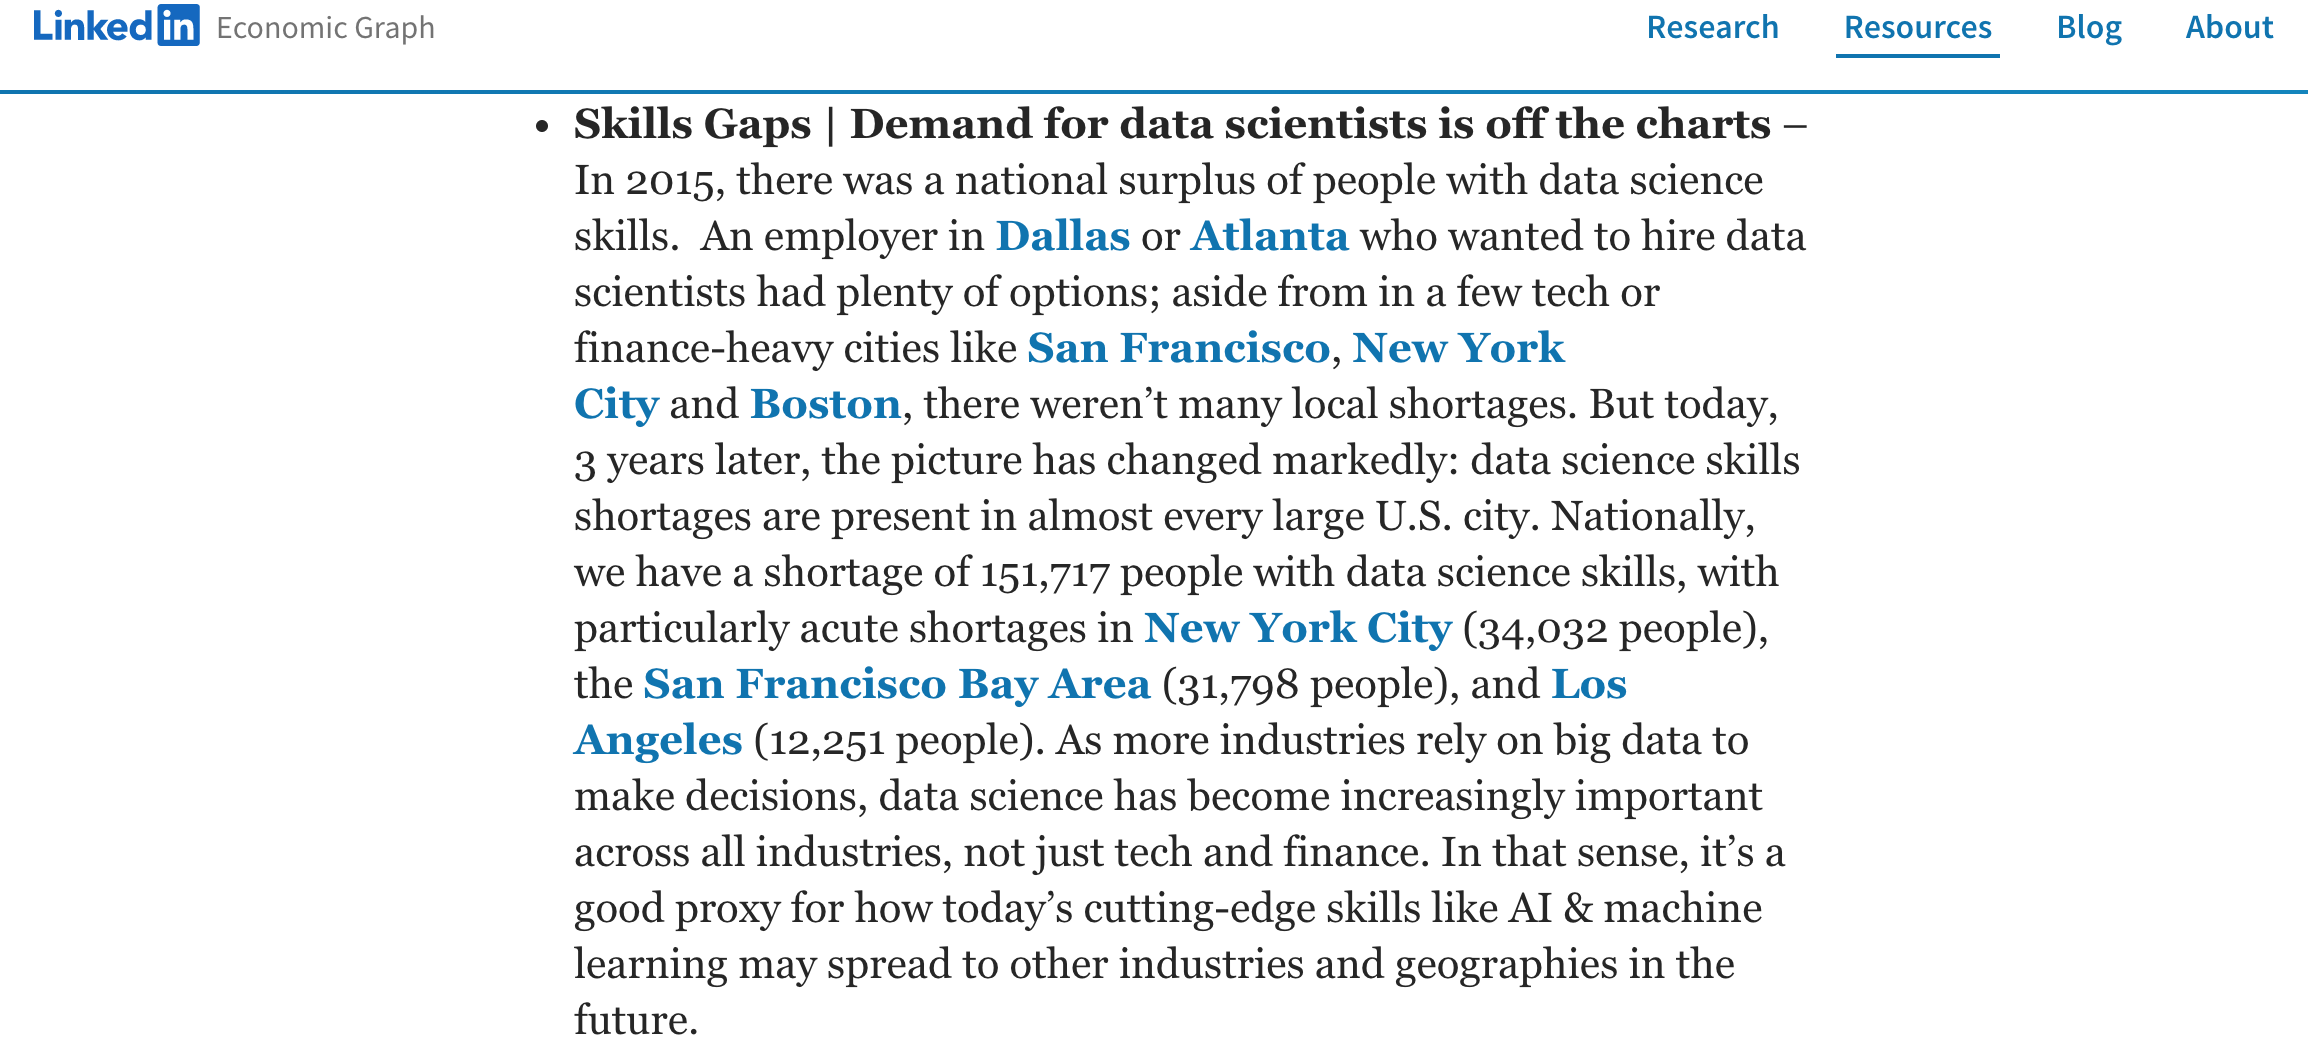
\includegraphics[width=0.7\linewidth]{figures/linkedin1} 

}

\caption{Linkedin economic report}\label{fig:unnamed-chunk-5}
\end{figure}

\begin{figure}

{\centering 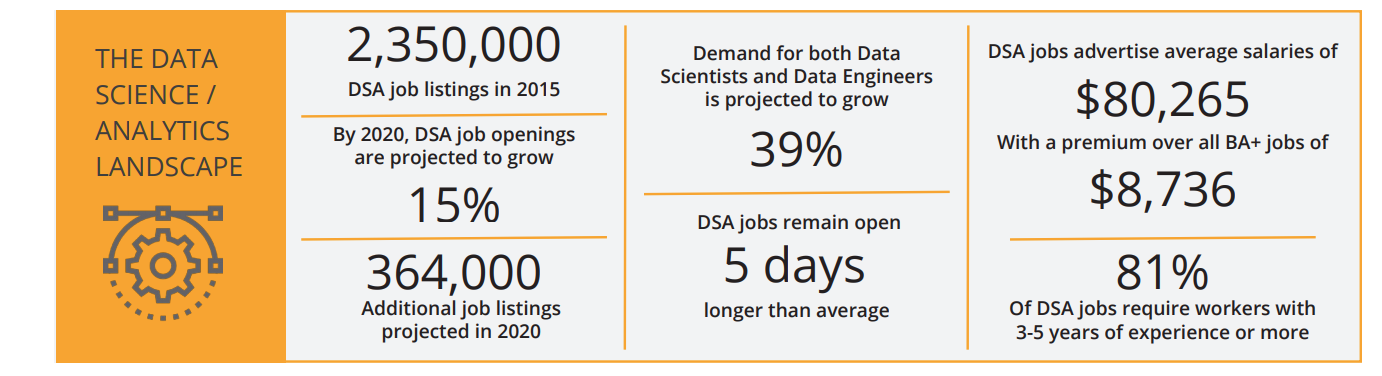
\includegraphics[width=0.7\linewidth]{figures/ibm} 

}

\caption{IBM}\label{fig:unnamed-chunk-6}
\end{figure}

class: clear

\begin{figure}

{\centering 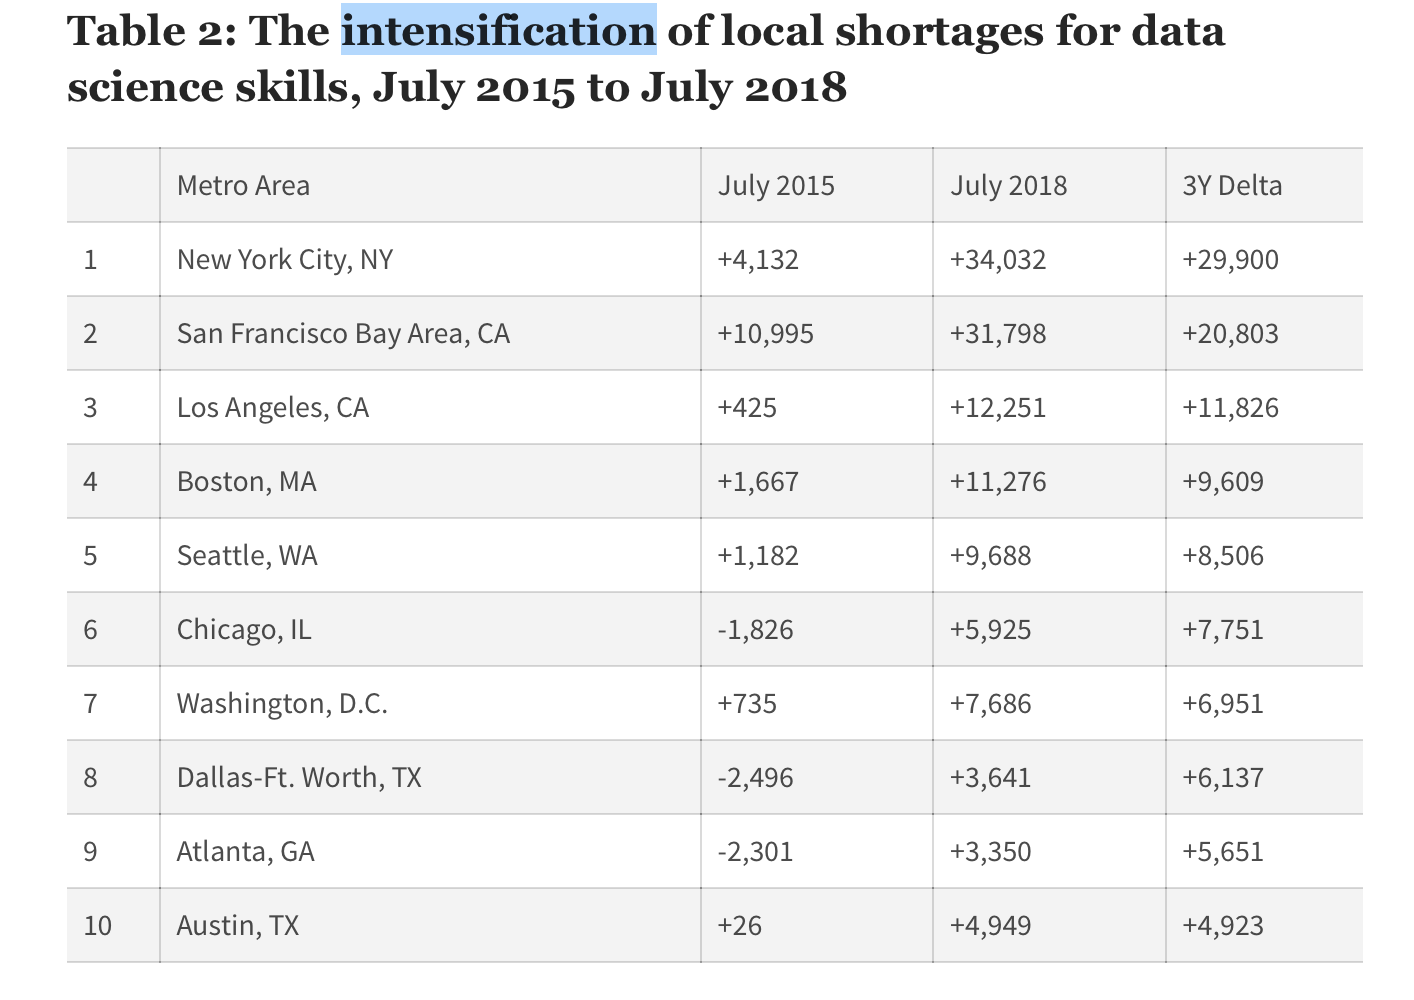
\includegraphics[width=0.7\linewidth]{figures/linkedin_shortage} 

}

\caption{Linkedin economic report}\label{fig:unnamed-chunk-8}
\end{figure}
\end{frame}

\begin{frame}{Word clouds, or crappy visuals ?}
\protect\hypertarget{word-clouds-or-crappy-visuals}{}
\begin{figure}

{\centering 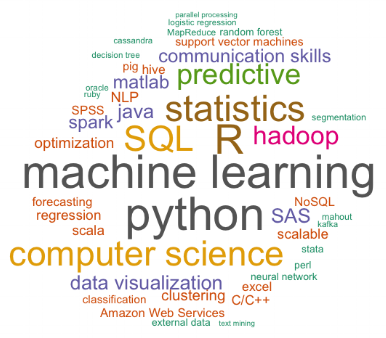
\includegraphics[width=0.7\linewidth]{figures/word_cloud_skills} 

}

\caption{http://www.kimberlycoffey.com/blog/2016/11/text-analysis}\label{fig:unnamed-chunk-10}
\end{figure}

class: clear

\begin{figure}

{\centering 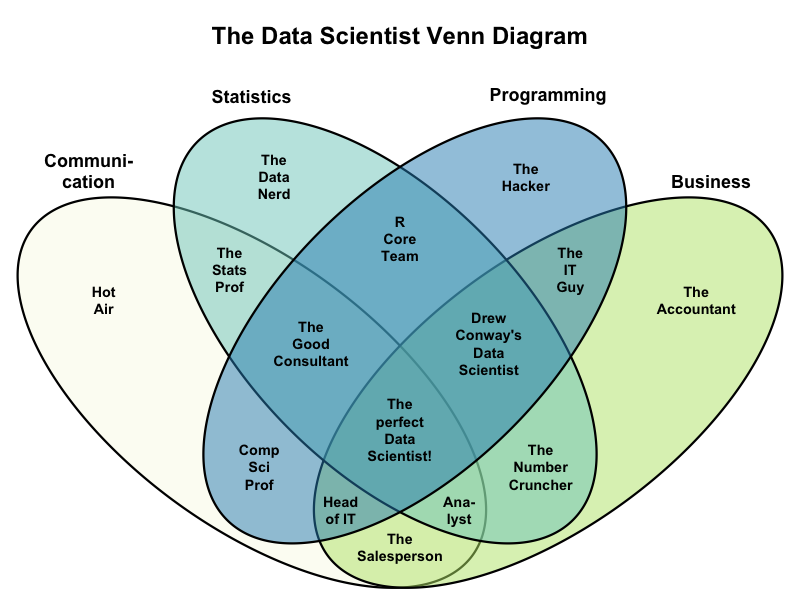
\includegraphics[width=0.8\linewidth]{figures/Venn} 

}

\caption{Figure from S. Kolassa}\label{fig:unnamed-chunk-13}
\end{figure}
\end{frame}

\begin{frame}{John Tukey FDA}
\protect\hypertarget{john-tukey-fda}{}
\begin{center}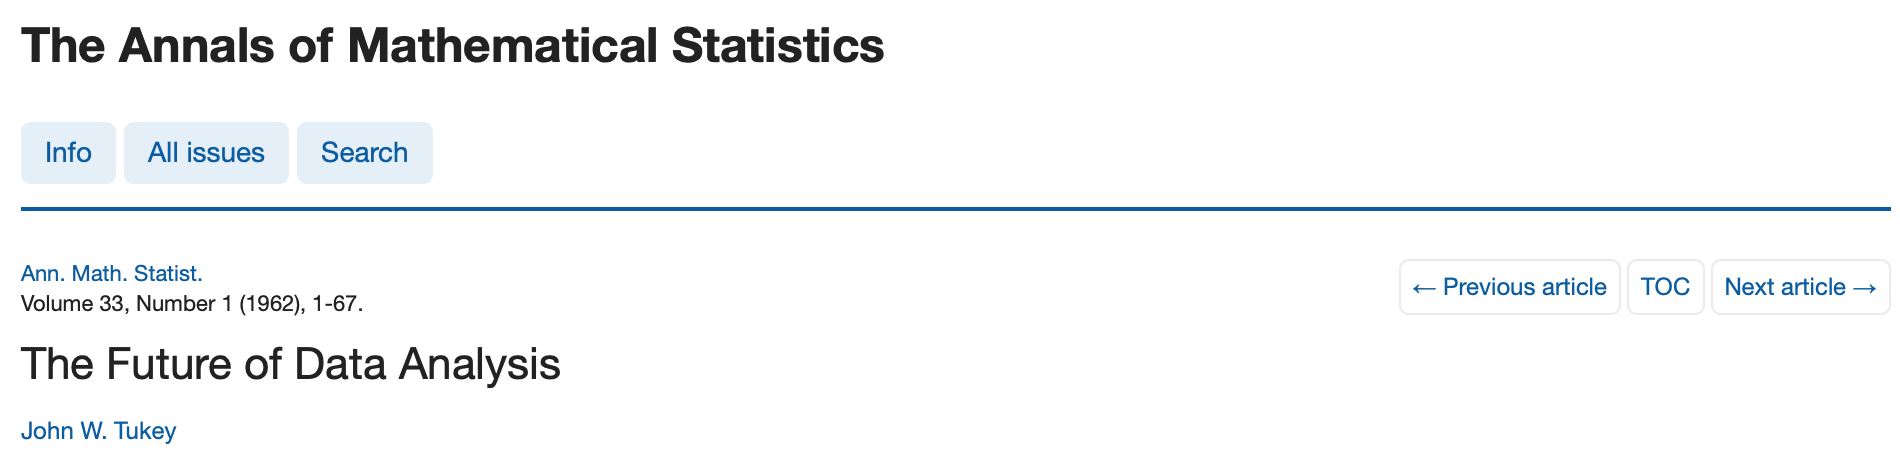
\includegraphics[width=0.7\linewidth]{figures/tukey1} \end{center}

\begin{center}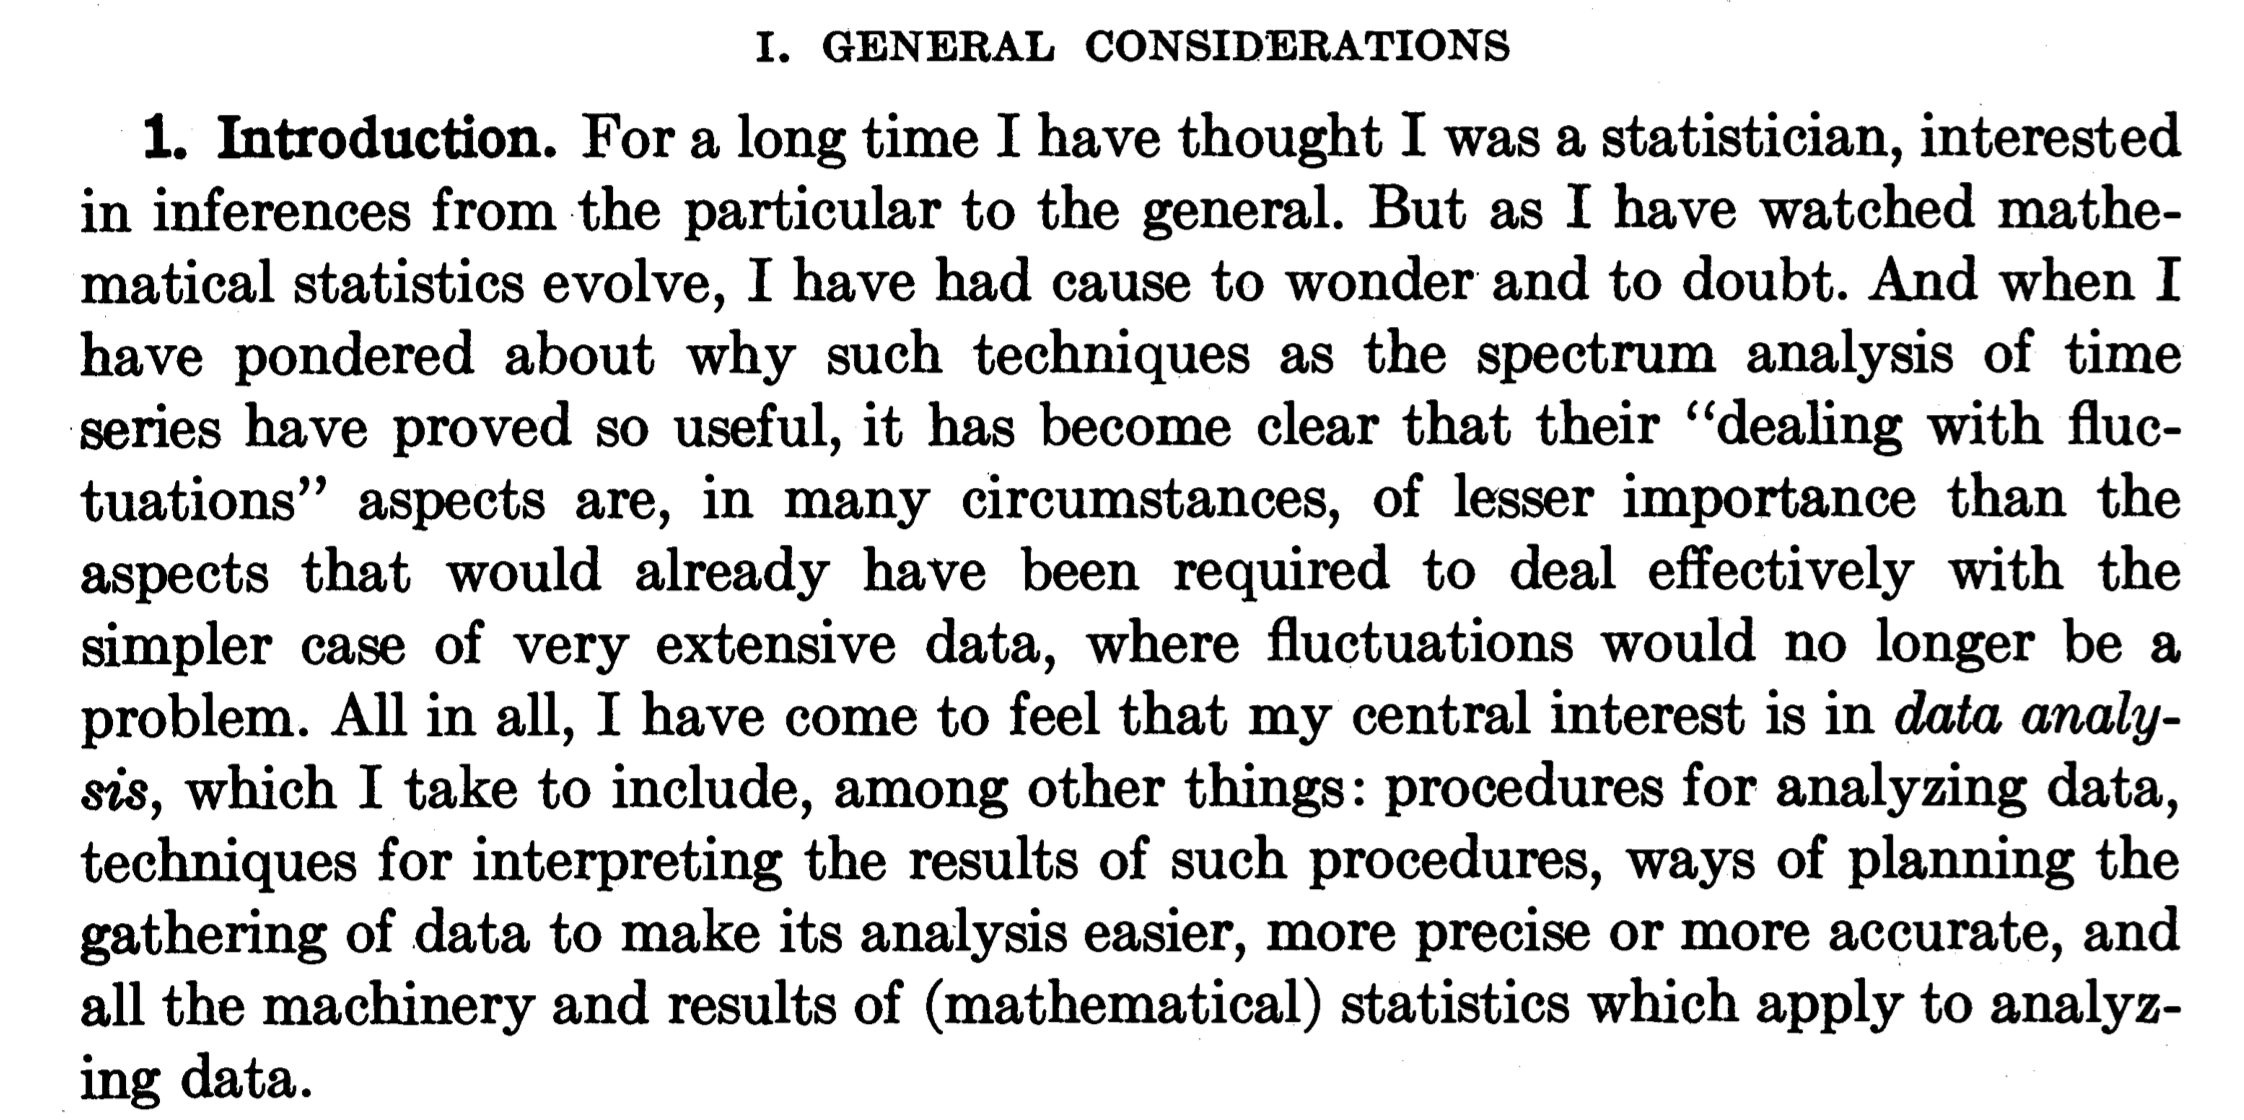
\includegraphics[width=0.7\linewidth]{figures/tukey2} \end{center}
\end{frame}

\begin{frame}{50 Years of Data Science}
\protect\hypertarget{years-of-data-science}{}
\begin{figure}

{\centering 
\includegraphics[width=0.7\linewidth]{figures/donoho} 

}

\caption{https://courses.csail.mit.edu/18.337/2015/docs/50YearsDataScience.pdf}\label{fig:unnamed-chunk-16}
\end{figure}
\end{frame}

\begin{frame}[fragile]{The R environment}
\protect\hypertarget{the-r-environment}{}
R is an integrated suite of software facilities for data manipulation,
calculation and graphical display. It includes + an effective data
handling and storage facility, + a suite of operators for calculations
on arrays, in particular matrices, + a large, coherent, integrated
collection of intermediate tools for data analysis, + graphical
facilities for data analysis and display either on-screen or on
hardcopy, and + a well-developed, simple and effective programming
language which includes conditionals, loops, user-defined recursive
functions and input and output facilities.

The term ``environment'' is intended to characterize it as a fully
planned and coherent system, rather than an incremental accretion of
very specific and inflexible tools, as is frequently the case with other
data analysis software. R can be extended (easily) via packages. There
are about eight packages supplied with the R distribution and many more
(\textgreater10,000) are available through the CRAN family of Internet
sites.

class: clear The previous Venn diagram was generated using the following
code taken from a
\href{https://datascience.stackexchange.com/questions/2403/data-science-without-knowledge-of-a-specific-topic-is-it-worth-pursuing-as-a-ca}{Stack
Exchange discussion}.

\begin{Shaded}
\begin{Highlighting}[]
\NormalTok{draw.ellipse \textless{}{-}}\StringTok{ }\ControlFlowTok{function}\NormalTok{(center,angle,semimajor,semiminor,radius,h,s,v,...) \{}
\NormalTok{    shape \textless{}{-}}\StringTok{ }\KeywordTok{rbind}\NormalTok{(}\KeywordTok{c}\NormalTok{(}\KeywordTok{cos}\NormalTok{(angle),}\OperatorTok{{-}}\KeywordTok{sin}\NormalTok{(angle)),}
                   \KeywordTok{c}\NormalTok{(}\KeywordTok{sin}\NormalTok{(angle),}\KeywordTok{cos}\NormalTok{(angle))) }\OperatorTok{\%*\%}\StringTok{ }\KeywordTok{diag}\NormalTok{(}\KeywordTok{c}\NormalTok{(semimajor,semiminor))}
\NormalTok{    tt \textless{}{-}}\StringTok{ }\KeywordTok{seq}\NormalTok{(}\DecValTok{0}\NormalTok{,}\DecValTok{2}\OperatorTok{*}\NormalTok{pi,}\DataTypeTok{length.out=}\DecValTok{1000}\NormalTok{)}
\NormalTok{    foo \textless{}{-}}\StringTok{ }\KeywordTok{matrix}\NormalTok{(center,}\DataTypeTok{nrow=}\DecValTok{2}\NormalTok{,}\DataTypeTok{ncol=}\KeywordTok{length}\NormalTok{(tt),}\DataTypeTok{byrow=}\OtherTok{FALSE}\NormalTok{)}\OperatorTok{+}
\StringTok{      }\NormalTok{shape}\OperatorTok{\%*\%}\NormalTok{(radius}\OperatorTok{*}\KeywordTok{rbind}\NormalTok{(}\KeywordTok{cos}\NormalTok{(tt),}\KeywordTok{sin}\NormalTok{(tt)))}
    \KeywordTok{polygon}\NormalTok{(foo[}\DecValTok{1}\NormalTok{,],foo[}\DecValTok{2}\NormalTok{,],}\DataTypeTok{col=}\KeywordTok{hsv}\NormalTok{(h,s,v,}\DataTypeTok{alpha=}\FloatTok{0.5}\NormalTok{),}\DataTypeTok{border=}\StringTok{"black"}\NormalTok{,...)}
\NormalTok{\}}
\NormalTok{name \textless{}{-}}\StringTok{ }\ControlFlowTok{function}\NormalTok{(x,y,label,}\DataTypeTok{cex=}\FloatTok{1.2}\NormalTok{,...) }\KeywordTok{text}\NormalTok{(x,y,label,}\DataTypeTok{cex=}\NormalTok{cex,...)}

\KeywordTok{png}\NormalTok{(}\StringTok{"\textasciitilde{}/Venn.png"}\NormalTok{,}\DataTypeTok{width=}\DecValTok{800}\NormalTok{,}\DataTypeTok{height=}\DecValTok{600}\NormalTok{)}
\NormalTok{    opar \textless{}{-}}\StringTok{ }\KeywordTok{par}\NormalTok{(}\DataTypeTok{mai=}\KeywordTok{c}\NormalTok{(}\DecValTok{0}\NormalTok{,}\DecValTok{0}\NormalTok{,}\DecValTok{0}\NormalTok{,}\DecValTok{0}\NormalTok{),}\DataTypeTok{lwd=}\DecValTok{3}\NormalTok{,}\DataTypeTok{font=}\DecValTok{2}\NormalTok{)}
        \KeywordTok{plot}\NormalTok{(}\KeywordTok{c}\NormalTok{(}\DecValTok{0}\NormalTok{,}\DecValTok{100}\NormalTok{),}\KeywordTok{c}\NormalTok{(}\DecValTok{0}\NormalTok{,}\DecValTok{90}\NormalTok{),}\DataTypeTok{type=}\StringTok{"n"}\NormalTok{,}\DataTypeTok{bty=}\StringTok{"n"}\NormalTok{,}\DataTypeTok{xaxt=}\StringTok{"n"}\NormalTok{,}\DataTypeTok{yaxt=}\StringTok{"n"}\NormalTok{,}\DataTypeTok{xlab=}\StringTok{""}\NormalTok{,}\DataTypeTok{ylab=}\StringTok{""}\NormalTok{)}
        \KeywordTok{draw.ellipse}\NormalTok{(}\DataTypeTok{center=}\KeywordTok{c}\NormalTok{(}\DecValTok{30}\NormalTok{,}\DecValTok{30}\NormalTok{),}\DataTypeTok{angle=}\FloatTok{0.75}\OperatorTok{*}\NormalTok{pi,}
                     \DataTypeTok{semimajor=}\DecValTok{2}\NormalTok{,}\DataTypeTok{semiminor=}\DecValTok{1}\NormalTok{,}\DataTypeTok{radius=}\DecValTok{20}\NormalTok{,}\DataTypeTok{h=}\DecValTok{60}\OperatorTok{/}\DecValTok{360}\NormalTok{,}\DataTypeTok{s=}\NormalTok{.}\DecValTok{068}\NormalTok{,}\DataTypeTok{v=}\NormalTok{.}\DecValTok{976}\NormalTok{)}
        \KeywordTok{draw.ellipse}\NormalTok{(}\DataTypeTok{center=}\KeywordTok{c}\NormalTok{(}\DecValTok{70}\NormalTok{,}\DecValTok{30}\NormalTok{),}\DataTypeTok{angle=}\FloatTok{0.25}\OperatorTok{*}\NormalTok{pi,}
                     \DataTypeTok{semimajor=}\DecValTok{2}\NormalTok{,}\DataTypeTok{semiminor=}\DecValTok{1}\NormalTok{,}\DataTypeTok{radius=}\DecValTok{20}\NormalTok{,}\DataTypeTok{h=}\DecValTok{83}\OperatorTok{/}\DecValTok{360}\NormalTok{,}\DataTypeTok{s=}\NormalTok{.}\DecValTok{482}\NormalTok{,}\DataTypeTok{v=}\NormalTok{.}\DecValTok{894}\NormalTok{)}
        \KeywordTok{draw.ellipse}\NormalTok{(}\DataTypeTok{center=}\KeywordTok{c}\NormalTok{(}\DecValTok{48}\NormalTok{,}\DecValTok{40}\NormalTok{),}\DataTypeTok{angle=}\FloatTok{0.7}\OperatorTok{*}\NormalTok{pi,}
                     \DataTypeTok{semimajor=}\DecValTok{2}\NormalTok{,}\DataTypeTok{semiminor=}\DecValTok{1}\NormalTok{,}\DataTypeTok{radius=}\DecValTok{20}\NormalTok{,}\DataTypeTok{h=}\DecValTok{174}\OperatorTok{/}\DecValTok{360}\NormalTok{,}\DataTypeTok{s=}\NormalTok{.}\DecValTok{397}\NormalTok{,}\DataTypeTok{v=}\NormalTok{.}\DecValTok{8}\NormalTok{)}
        \KeywordTok{draw.ellipse}\NormalTok{(}\DataTypeTok{center=}\KeywordTok{c}\NormalTok{(}\DecValTok{52}\NormalTok{,}\DecValTok{40}\NormalTok{),}\DataTypeTok{angle=}\FloatTok{0.3}\OperatorTok{*}\NormalTok{pi,}
                     \DataTypeTok{semimajor=}\DecValTok{2}\NormalTok{,}\DataTypeTok{semiminor=}\DecValTok{1}\NormalTok{,}\DataTypeTok{radius=}\DecValTok{20}\NormalTok{,}\DataTypeTok{h=}\DecValTok{200}\OperatorTok{/}\DecValTok{360}\NormalTok{,}\DataTypeTok{s=}\NormalTok{.}\DecValTok{774}\NormalTok{,}\DataTypeTok{v=}\NormalTok{.}\DecValTok{745}\NormalTok{)}
\end{Highlighting}
\end{Shaded}

\#Course overview

\begin{figure}

{\centering 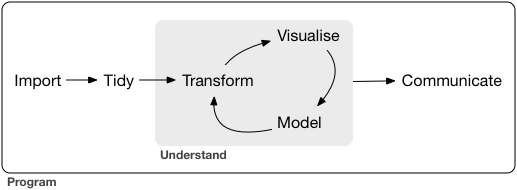
\includegraphics[width=0.7\linewidth]{figures/data_science_pipeline} 

}

\caption{https://r4ds.had.co.nz}\label{fig:unnamed-chunk-19}
\end{figure}

We will cover the following topics + Data wrangling and tidying with
dplyr and tidyr (\textbf{R} libraries) + Data visualization with ggplot2
(\textbf{R} library) + Hitch-hiker guide to SQL. + Linear regression and
scatterplot smoothing. + Classification, \(k\)-NN, linear/quadratic
discriminant analysis, logistic regression. + Decision trees, support
vectors machine. + principal components analysis, multidimensional
scaling, clustering.

class: clear

\begin{block}{Homework policy}
\protect\hypertarget{homework-policy}{}
The class has, with high probability, 7 homework assignments. Late
homework submissions will be penalized. In particular + Less than 24
hours late: 20\% penalty towards total points. + Between 24 hours and 48
hours late: 40\% penalty towards total points + Between 48 hours and 72
hours late: 75\% penalty towards total points + More than 72 hours late:
Not graded.
\end{block}

\begin{block}{Term paper}
\protect\hypertarget{term-paper}{}
\end{block}

\begin{block}{For the final project, the students will work either
individually or in a team of no more than three members. Each individual
or group will complete a data analysis and write a short report (10
pages or less) summarizing the work.~The report should provide a clear
description of the dataset, the scientific questions of interest, the
technical approach used to address or answer these questions, and state
what conclusions, if any, can be derived from the analysis.}
\protect\hypertarget{for-the-final-project-the-students-will-work-either-individually-or-in-a-team-of-no-more-than-three-members.-each-individual-or-group-will-complete-a-data-analysis-and-write-a-short-report-10-pages-or-less-summarizing-the-work.-the-report-should-provide-a-clear-description-of-the-dataset-the-scientific-questions-of-interest-the-technical-approach-used-to-address-or-answer-these-questions-and-state-what-conclusions-if-any-can-be-derived-from-the-analysis.}{}
class: clear \#\#\# Choice of programming language The use of R for
homework assignments and final project is encouraged, but not required.
You are free to use any programming language of your choice. Note
however that your TA and course instructor might not be able to
help/answer your inquiry should you choose to use a different
programming language.

\begin{block}{Grading disputes}
\protect\hypertarget{grading-disputes}{}
Your assignment and exams score will be entered and stored on the Moodle
page. You are responsible for keeping track of your scores and to notify
the course instructor should there be any missing grades or
discrepancies. Your exams will be returned to you after they had been
graded. Please keep all returned exams. Grading dispute for an
assignment will be considered only if the dispute is initiated within
one week of the grade being entered. Grading dispute for an exam should
be made within 72 hours of the exam being returned. A grading dispute
might entail a regrading of the whole submission.

class: clear \#\#\#Ethics The strength of the university depends on
academic and personal integrity. In this course, you must be honest and
truthful. Students are permitted and indeed encouraged to discuss
lecture materials and homework problems with one another, but it is
expected that the writing up of answers will be done privately. Copying
by one student of another student's homework solutions is considered an
ethics violation in this course. Specifically, please do not share code
or output; please do not access or use solutions from any source before
your homework assignment is submitted. More information about university
misconduct policies are available at +
\href{http://policies.ncsu.edu/policy/pol-11-35-01}{Code of student
conduct} + \href{http://policies.ncsu.edu/policy/pol-11-35-01}{Academic
honesty}

\#\#\#Students with Disabilities Reasonable accommodations will be made
for students with verifiable disabilities. In order to take advantage of
available accommodations, students must register with the Disability
Resource Office at Holmes Hall, Suite 304, Campus Box 7509,
919-515-7653. For more information on NC State's policy on working with
students with disabilities, please see the
\href{https://policies.ncsu.edu/regulation/reg-02-20-01/}{Academic
Accommodations for Students with Disabilities}
\end{block}
\end{block}
\end{frame}

\end{document}
